\documentclass[11pt]{article}

\usepackage[margin=1in]{geometry}
\usepackage{amsmath}
\usepackage{amsfonts}
\usepackage{algorithm}
\usepackage{algpseudocode}
\usepackage{booktabs}
\usepackage{graphicx}
\usepackage[hidelinks]{hyperref}

\algrenewcommand{\algorithmiccomment}[1]{\hfill\textit{// #1}}

\title{Gradient-informed sampling for VPD}
\author{Chandan Sreedhara \and Christian Franssen}
\date{April 2026}

\begin{document}
\maketitle

\section{Introduction}

Stochastic Parameter Decomposition (SPD) \cite{bushnaq2025stochasticparameterdecomposition}
decomposes neural network parameters into sparsely used components via the objective
\begin{align*}
    \mathcal{L}_{\mathrm{SPD}}
    = \mathcal{L}_{\mathrm{faithfulness}}
    + \sum_{i=1}^n \beta_i \mathcal{L}^{(i)}_{\mathrm{recon}}
    + \beta_{n+1} \mathcal{L}_{\mathrm{importance\text{-}minimality}}.
\end{align*}
Its dominant cost comes from reconstruction losses, which evaluate reconstruction error
under different component masks. VPD adds adversarial reconstruction: several steps of
projected gradient ascent find a high-loss mask before the model is optimized against it
\cite{bushnaq2026interpreting}.

This report asks whether the stochastic reconstruction terms can use their available
gradient information more effectively. They currently sample masking sources uniformly.
We propose \textbf{Gradient-Informed Sampling (GIS)}, which biases a stochastic draw
toward components with high reconstruction-loss sensitivity. Our main claim is narrow:
GIS finds higher-loss masks than uniform sampling at low marginal cost. PGD is included
as an optimization-based reference, not as a competing sampler.

\section{Background}

The reconstruction objective can be written as
\begin{align}
\label{eq:abl_req}
    \min_{U,V,\theta}\;\mathbb{E}_{r\sim p}
    \left[D\!\left(f\!\left(x\mid W'(x,r)\right),f(x\mid W)\right)\right],
\end{align}
where $U$ and $V$ contain the subcomponents, $\theta$ parameterizes the causal
importance functions $g$, and $p$ has full support on $[0,1]^{C\times L}$.
Here $C$ is the number of components and $L$ the number of layers; the remaining
notation follows the SPD paper. The practical sum of reconstruction losses approximates
this intractable objective. Efficient training therefore benefits from sources $r$ that
make large contributions to its integrand; adversarial reconstruction targets the same
quantity through an inner optimization loop.

\section{Methodology}

GIS reuses the sensitivity from one reconstruction term,
$\mathcal L_{\mathrm{recon}}^{(1)}$, to sample the next. For component $c$ in layer $l$,
it assigns weight
\begin{align}
\label{eq:weights}
    p_c^l =
    \frac{\left|\partial\mathcal L_{\mathrm{recon}}^{(1)}/\partial g_c^l\right|^k}
    {\sum_{c'}\left|\partial\mathcal L_{\mathrm{recon}}^{(1)}/
    \partial g_{c'}^l\right|^k+\varepsilon}.
\end{align}
It then draws $r_c^l\sim U[0,1]$ and constructs
\begin{align}
\label{eq:mask}
    \widetilde r_c^l=(1-p_c^l)r_c^l,
    \qquad
    m_c^l=g_c^l+(1-g_c^l)\widetilde r_c^l.
\end{align}
Large gradient magnitude therefore causes stronger ablation, while $k$ controls how
strongly the sampler concentrates on the largest gradients. When the first loss's
forward pass is already present, GIS adds no forward pass; obtaining the sensitivity
requires one partial backward through the retained graph and temporary storage of the
component gradients.

\begin{algorithm}[H]
\caption{Gradient-Informed Sampling}
\label{alg:gis}
\begin{algorithmic}[1]
\Require causal importance parameters $\theta$, training data $\mathcal X$, temperature $k$
\For{each outer training step}
    \State Sample $x$ and compute $y^*=f_{\mathrm{target}}(x)$
    \State Compute $\{g_c^l(\theta)\}=\Gamma_\theta(x)$
    \State Compute $\mathcal L_{\mathrm{recon}}^{(1)}$ with a random mask
    \State Compute $p_c^l$ using Equation~\ref{eq:weights}
    \State Draw $r_c^l\sim U[0,1]$ and construct $\widetilde r_c^l,m_c^l$ using Equation~\ref{eq:mask}
    \State Compute $\hat y=f(x;W'(x,\{m_c^l\}))$
    \State $\theta\gets\theta-\eta\nabla_\theta
    [\mathcal L_{\mathrm{recon}}^{(1)}+\mathcal L_{\mathrm{recon\text{-}subset}}(\hat y,y^*)]$
\EndFor
\end{algorithmic}
\end{algorithm}

\section{Direct sampler benchmark}
\label{sec:sampler_benchmark}

We first isolate the sampling question from training. A \texttt{resid\_mlp2}
ComponentModel is trained with uniform sampling and frozen at the final checkpoint.
Uniform, GIS, and PGD then see the same evaluation batches and use the same mask
construction. We report the reconstruction error induced by each mask,
$\Delta\mathcal L_{\mathrm{recon}}$; larger values indicate harder masks.

PGD starts from a uniform source and performs sign-gradient ascent on this same
objective with step size $0.5$. Its results calibrate the scale of the GIS improvement;
they are not a like-for-like sampler comparison. The weight-delta mask remains random
in every arm so that only the component source changes.

\begin{table}[ht]
\centering
\small
\begin{tabular}{lrrrr}
\toprule
Method & Marginal fwd/bwd$^\dagger$ & $\Delta\mathcal L_{\mathrm{recon}}$
& vs. uniform & PGD-20 headroom \\
\midrule
Uniform       & $0/0$   & $1.1826\times10^{-4}$ & $1.00\times$ & 0.0\% \\
GIS, $k=1$    & $0/1$   & $1.3454\times10^{-4}$ & $1.14\times$ & 1.1\% \\
GIS, $k=2$    & $0/1$   & $1.5131\times10^{-4}$ & $1.28\times$ & 2.2\% \\
GIS, $k=4$    & $0/1$   & $1.5858\times10^{-4}$ & $1.34\times$ & 2.6\% \\
GIS, $k=8$    & $0/1$   & $1.6222\times10^{-4}$ & $1.37\times$ & 2.9\% \\
\midrule
PGD, 1 step   & $1/1$   & $5.3078\times10^{-4}$ & $4.49\times$ & 27.1\% \\
PGD, 2 steps  & $2/2$   & $8.1299\times10^{-4}$ & $6.87\times$ & 45.6\% \\
PGD, 5 steps  & $5/5$   & $1.3021\times10^{-3}$ & $11.01\times$ & 77.6\% \\
PGD, 20 steps & $20/20$ & $1.6432\times10^{-3}$ & $13.89\times$ & 100.0\% \\
\bottomrule
\end{tabular}
\caption{Final-checkpoint results over three seeds and 20 paired batches per seed.
The GIS ratio varied by less than $\pm0.01$ across seeds. ``PGD-20 headroom'' is
$(\Delta\mathcal L-\Delta\mathcal L_{\mathrm{uniform}})/
(\Delta\mathcal L_{\mathrm{PGD20}}-\Delta\mathcal L_{\mathrm{uniform}})$.
$^\dagger$Marginal cost when GIS reuses the forward pass of an existing reconstruction
loss. The standalone benchmark explicitly computes this signal.}
\label{tab:benchmark}
\end{table}

GIS consistently finds harder masks than uniform sampling, and the advantage increases
from $1.14\times$ at $k=1$ to $1.37\times$ at $k=8$. The result establishes the intended
mechanism: gradient magnitude contains useful information for a subsequent stochastic
draw.

The same table also bounds the importance of this result. Twenty-step PGD finds
$13.89\times$ the uniform reconstruction loss, while GIS recovers only 2.9\% of the
gap between uniform and PGD-20. Even one PGD step is much stronger than GIS, at the cost
of an additional forward pass. GIS should therefore be evaluated against uniform, not
presented as an alternative to adversarial optimization.

\section{Training results}

Figure~\ref{fig:training-results} compares two uniform baselines, GIS, and PGD on
\texttt{resid\_mlp2}. GIS substantially reduces target-solution error and adversarial
reconstruction loss relative to both uniform baselines. PGD achieves the lowest
\texttt{PGDReconLoss}, but also the highest importance-minimality loss; GIS lies between
uniform sampling and PGD on both measures. The training metrics show the same broad
ordering: GIS incurs a harder training objective than uniform sampling but remains less
aggressive than PGD.

In the hyperparameter sweep, the best GIS run reaches an evaluation PGD reconstruction
loss of $1.86\times10^{-4}$ and target-solution error of $18.6$, versus
$1.57\times10^{-4}$ and $12.0$ for PGD. PGD with five steps takes $2976$ seconds,
compared with $2121$--$2149$ seconds for GIS, or about $1.4\times$ longer
(Figure~\ref{fig:training-results}, bottom, for the wall-clock comparison).

All GIS training runs use $k=1$, the implementation default and the weakest setting in
Table~\ref{tab:benchmark}. The frozen-model result therefore does not yet establish that
harder GIS draws train a better decomposition. It establishes only that GIS can find
harder draws cheaply.

\begin{figure}[p]
    \centering
    \textbf{(a) Evaluation and training metrics}\par\smallskip
    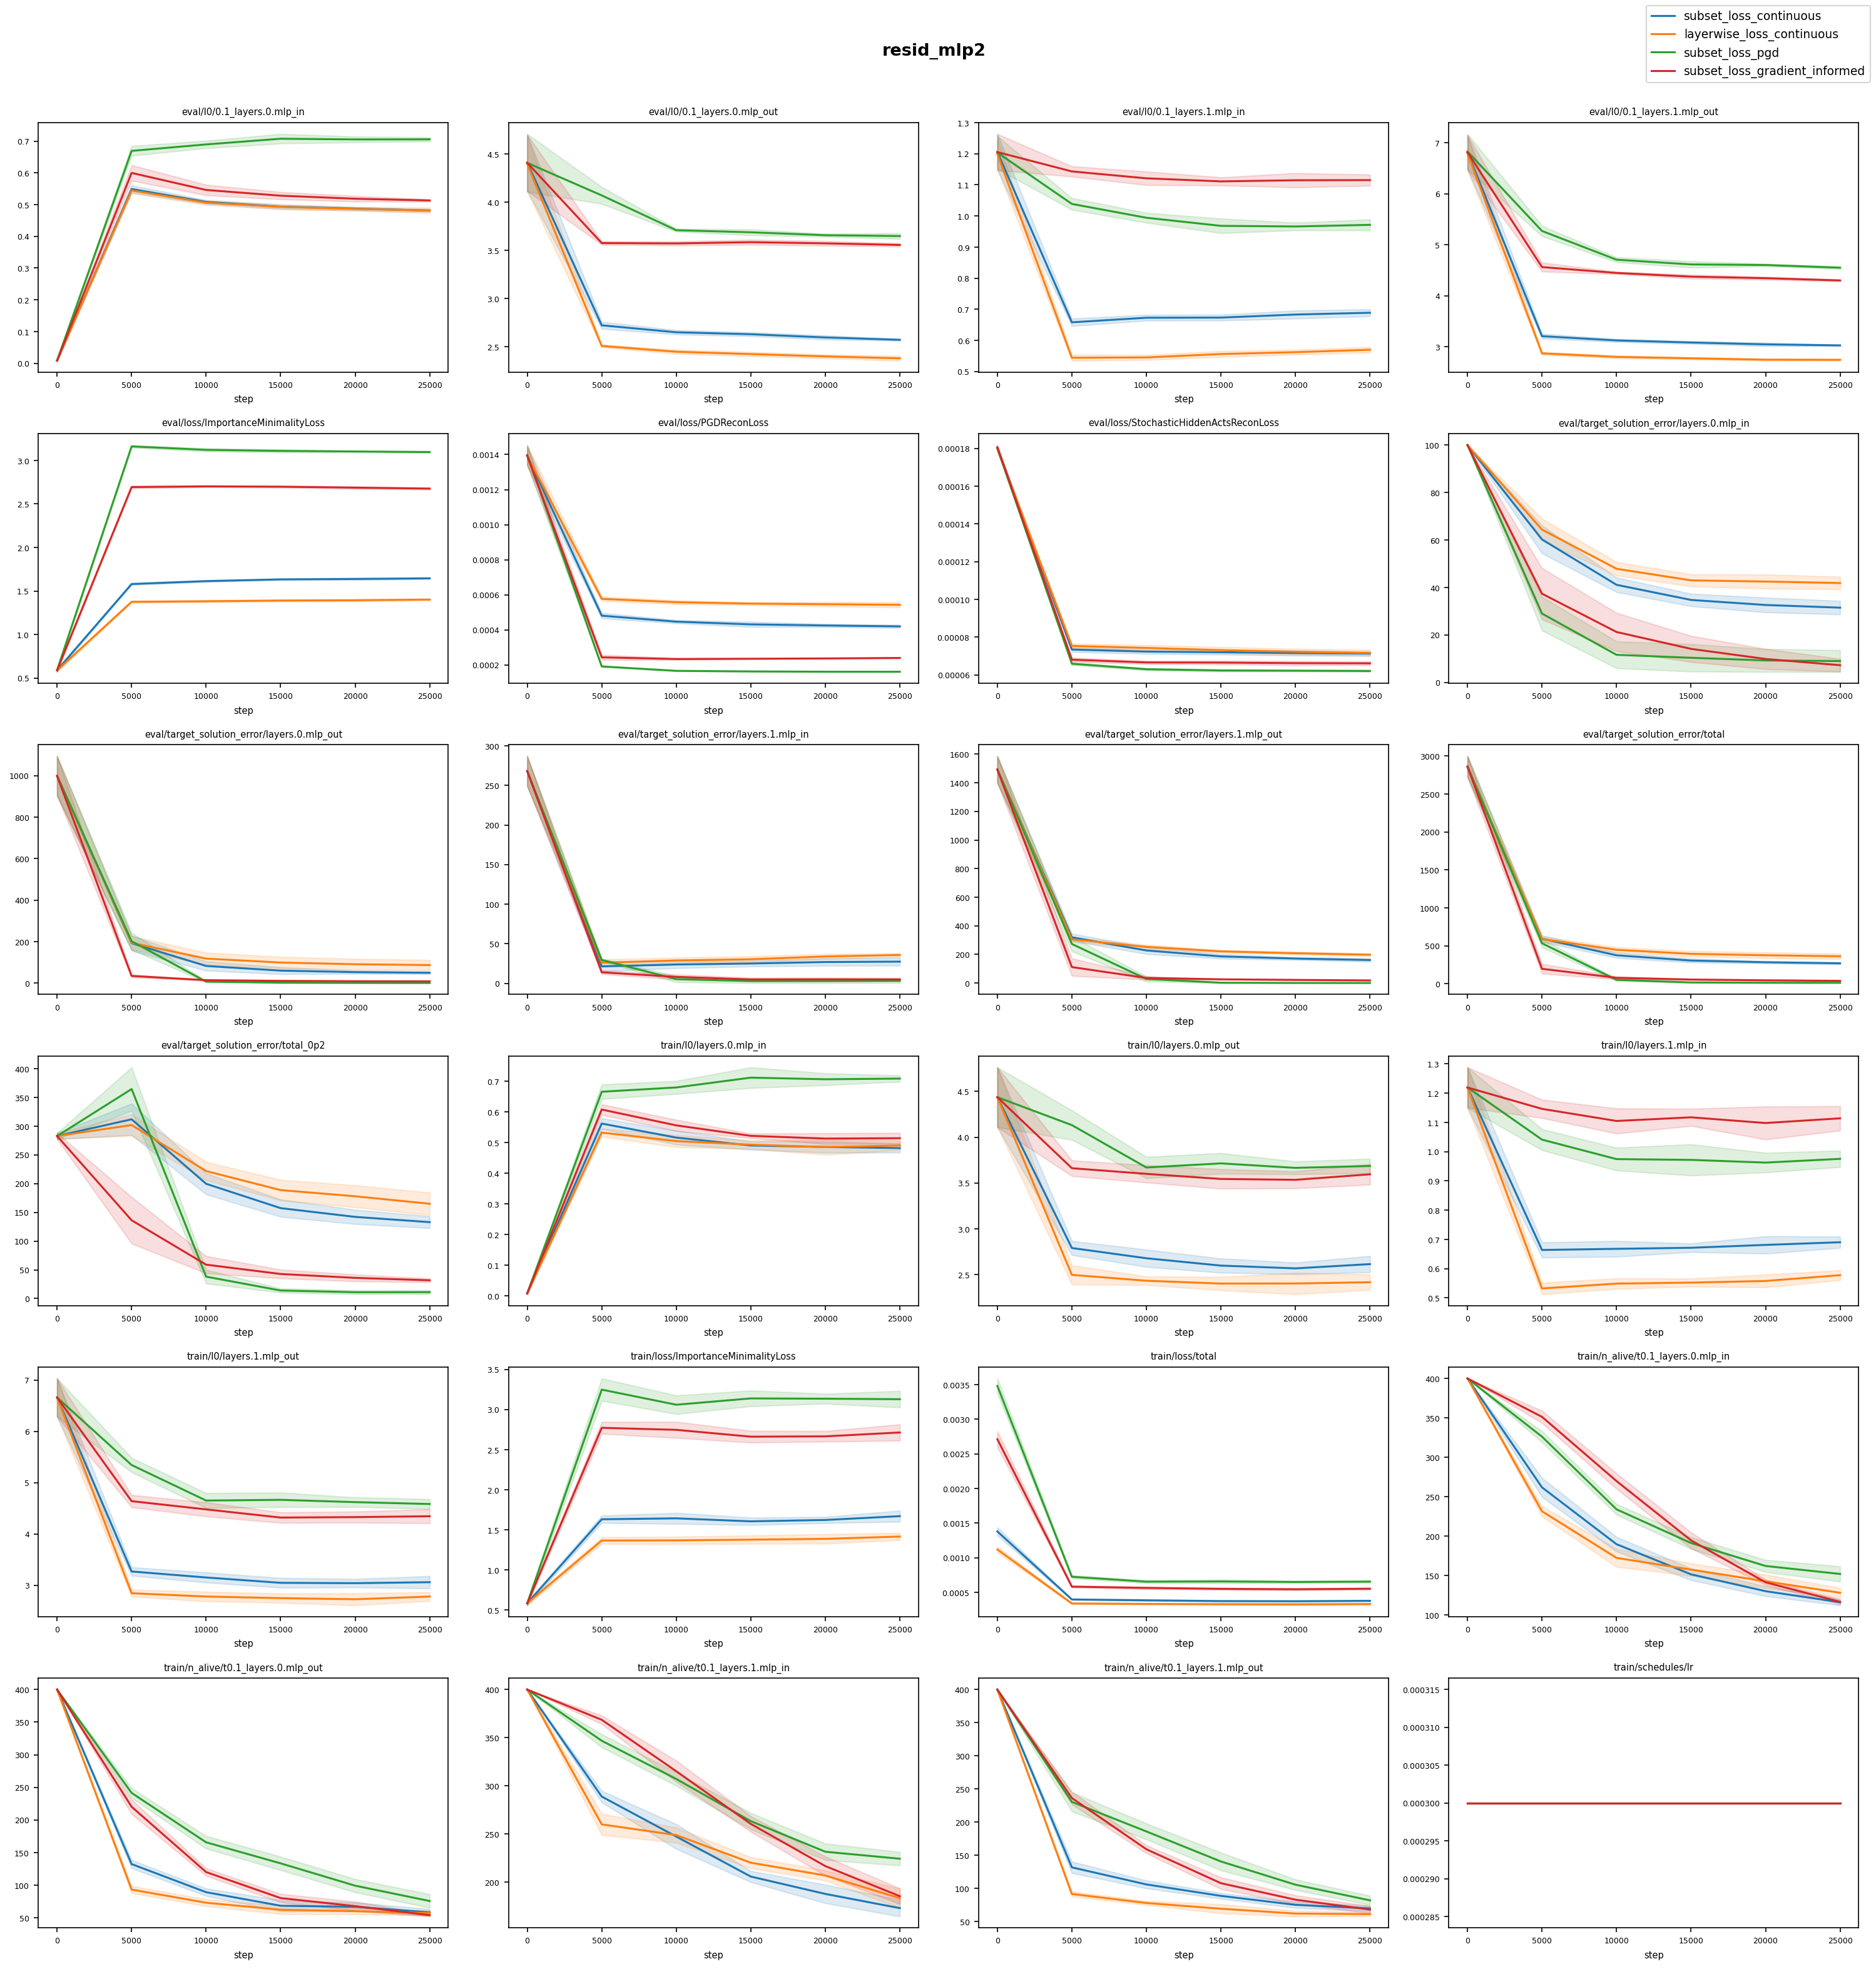
\includegraphics[width=0.80\textwidth]{resid_mlp2_comparision.png}

    \medskip
    \textbf{(b) Wall-clock training time}\par\smallskip
    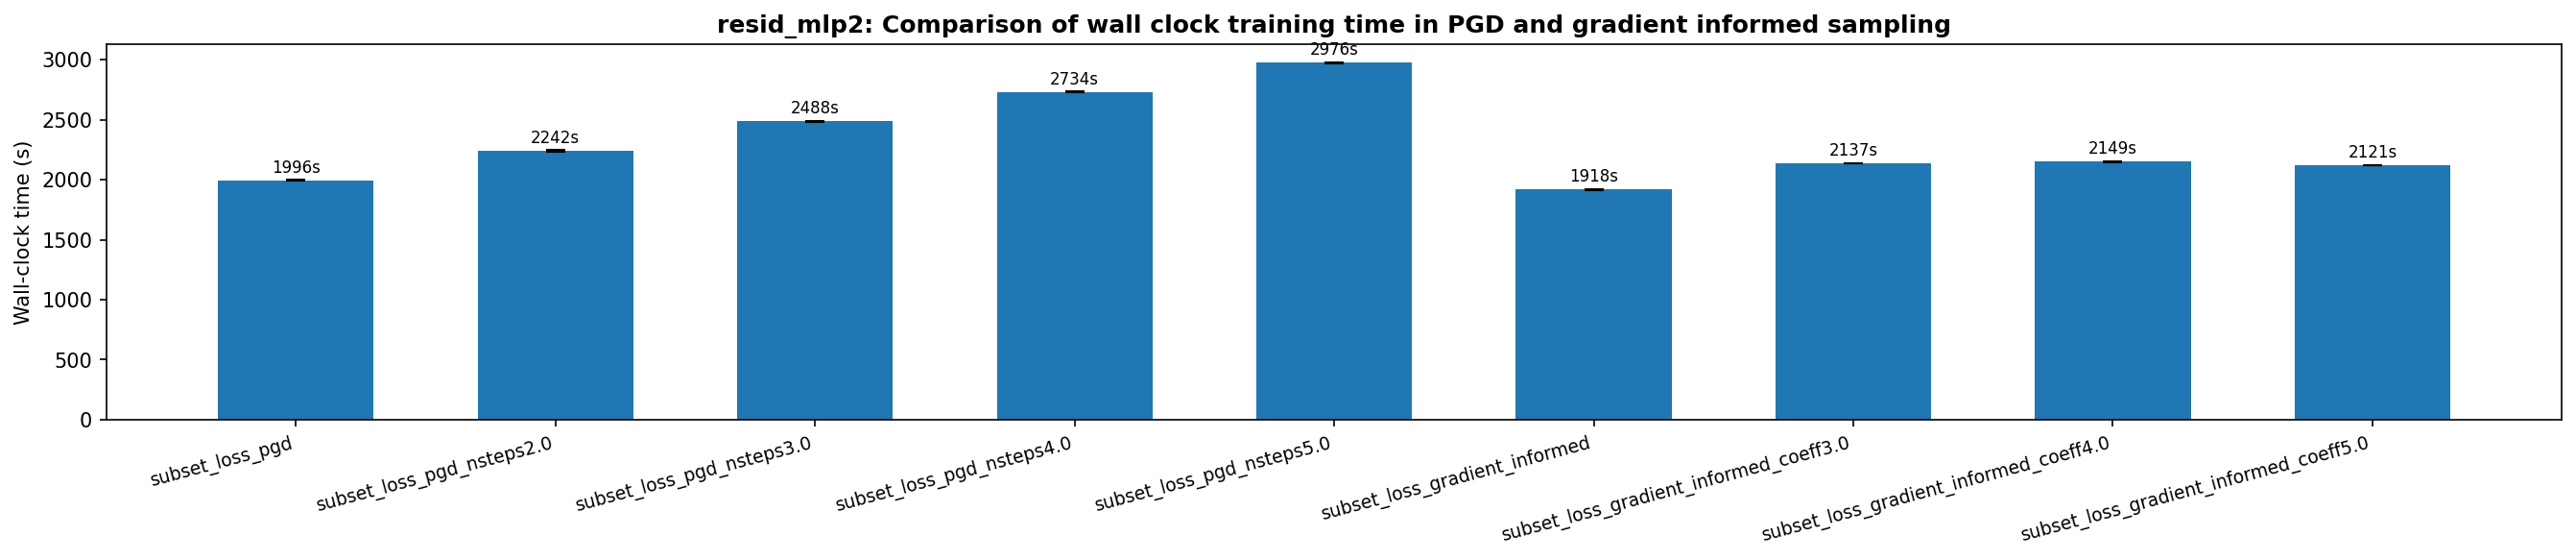
\includegraphics[width=0.95\textwidth]{resid_mlp2_pgd_vs_gradient-informed_wallclock.png}
    \caption{Training results on \texttt{resid\_mlp2}. (a) Uniform sampling with
    subset or layerwise losses, GIS, and PGD across evaluation and training metrics;
    bands show variation across seeds. (b) Training time for PGD step counts and GIS
    loss coefficients. GIS cost is nearly flat in its coefficient, whereas PGD cost
    increases with the number of inner steps.}
    \label{fig:training-results}
\end{figure}

\section{Proposed use in VPD}

VPD's merged reconstruction loss already combines adversarial and uniformly sampled
sources. Our results suggest that its uniform portion may be made more informative
without changing the adversarial portion. We would therefore value the VPD authors'
guidance on the following question:

\begin{quote}
\emph{Would replacing VPD's uniform mask sources with GIS sources be useful while
leaving its PGD sources unchanged? If so, which model and configuration would provide
the most informative first experiment?}
\end{quote}

The corresponding ablation would be
\begin{equation*}
 \text{PGD + uniform} \quad\text{vs.}\quad \text{PGD + GIS},
\end{equation*}
at matched PGD steps, loss coefficients, and seeds, with wall-clock time and memory
reported separately. Evaluation should report final decomposition metrics and
adversarial reconstruction loss.

Three uncertainties remain. First, biasing the stochastic half may reduce the broad
coverage for which it was included. Second, harder masks on a frozen model need not
provide a better training signal. Third, the cost of the partial backward pass and its
activation memory has not been measured at language-model scale.

\section{Conclusion}

GIS is a reliable improvement over uniform sampling in the direct test: it recovers up
to 37\% more reconstruction loss with no additional forward pass when its gradient
signal is reused. The gain is small relative to PGD and does not justify replacing PGD.
The supported next step is narrower: test GIS in place of the uniform draws that VPD
already uses alongside PGD.

\begin{thebibliography}{2}
\bibitem{bushnaq2025stochasticparameterdecomposition}
L.~Bushnaq, D.~Braun, and L.~Sharkey.
\newblock \emph{Stochastic Parameter Decomposition}.
\newblock 2025. \url{https://arxiv.org/abs/2506.20790}.

\bibitem{bushnaq2026interpreting}
J.~Bushnaq et al.
\newblock \emph{Interpreting language models with VPD}.
\newblock Goodfire Research, 2026.
\newblock \url{https://static.goodfire.ai/vpd-blog-post/post.md}.
\end{thebibliography}

\end{document}
